\documentclass[11pt, oneside]{amsart}   	% use "amsart" instead of "article" for AMSLaTeX format
\usepackage{geometry}  
\usepackage{hyperref}  
\geometry{letterpaper}                   		% ... or a4paper or a5paper or ... 
%\geometry{landscape}                		% Activate for for rotated page geometry
%\usepackage[parfill]{parskip}    		% Activate to begin paragraphs with an empty line rather than an indent
\usepackage{graphicx}				% Use pdf, png, jpg, or eps� with pdflatex; use eps in DVI mode
								% TeX will automatically convert eps --> pdf in pdflatex		
\usepackage{amssymb}
\usepackage{listings}

\title{CS 325: Project 2}
\author{Group 29: Jacob Mastel, Robert Erick, Cera Olson}
\date{10 May 2015}							% Activate to display a given date or no date

\begin{document}
\maketitle
\newpage{}
\tableofcontents
\newpage{}

\section{Changeslow Algorithm}
The changeslow algorithm can also be called brute force or divide and conquer. We used the algorithm to find the minimum number of coins to make i and $K-i$ cents. 
\subsection{Pseudocode\newline}
This is the pseudocode for the Changeslow Algorithm. It completes the requirement for Question 2. 
\lstinputlisting[language=Python]{pseudocode/pseudocode_a1.txt}

\section{Greedy Algorithm}
The greedy algorithm starts with the largest values and goes through the lower values ignored to determine the lowest number of coins to make i and $K-i$ cents. 
\subsection{Pseudocode\newline}
This is the pseudocode for the Greedy Algorithm. It completes the requirement for Question 2. 
\lstinputlisting[language=Python]{pseudocode/pseudocode_a2.txt}

\section{Dynamic Programming}
Dynamic programming stores the calculated values to reduce the running time for larger values. 
\subsection{Pseudocode\newline}
This is the pseudocode for the Dynamic Programming. It completes the requirement for Question 2. 
\lstinputlisting[language=Python]{pseudocode/pseudocode_a3.txt}

\section{Questions}
\subsection{Describe, in words, how you fill in the dynamic programming table in changedp. Justify why is this a valid way to fill the table?\newline}

The methodology for filling the dynamic programming table is as follows:
\par
First a table is constructed with columns [0..value we're looking for], interval of 1.  The rows are [0..number of coins we have].  Let the indexes be r and c so that a each cell has coordinate (r, c).  Let each row have a value of rv associated with the value for each coin, in increasing order.  Let each column have a value cv associated with the values for each column, [0..value we're looking for]. c and cv have the same range.
\par
If it is the first cell of the table, (0,0), the value is 0:
\par
Otherwise, for the cells in the first row, the value of each cell c1 is the value of the cell c2 which occurs rv intervals prior, plus 1 (where rv is the row's value).  Example:  if row 0 represents a 1 cent coin, its "row value" is 1.  Therefore, for cell (0,1), it's value will be the value of cell to its left by 1 (rv), which is cell (0,0), which has a value of 0, and this is increased by 1.
\par
Otherwise, for cells in the lower rows, at the beginning of the row:  all cells from (0,r) (where are is the row) inward are carried down from the cell immediately above each.  Thus, which cv<rv for each cell, carry down from above.
\par
Otherwise, for cells in the endings of each row: compute the minimum of the value immediately above with the value compared with the value of the cell to the left rv hops, plus 1.   That is, the minimum of a) value of cell(r-1,c) or b) (value of cell$(r,c-rv))+1$.
\par
This methodology is correct.  Firstly, smaller problems are being solved starting with the smallest rows and starting with the smallest values within those rows, working from the top left corner of the table down to the bottom right corner.  The process builds from smallest solutions to greatest.  
\par
Secondly, populating the top row gives solutions as if the 1 coin were the only coin available.  Each solution on the left helps develop the answer to its right.  However, the subsequent rows are all populated thusly:  the first portion of the row has solutions too small for that row's coin to solve, so the optimal solution from above is copied down.  The second portion of the row is populated by using the matching optimal solution to the left plus that row's coin, or the optimal solution above.  This process allows new information to be introduced (the new, higher valued coin) and used in an optimal solution, or to use the solution above if it is superior.  Each successive row can, potentially, copy down the optimal solutions developed by the lower valued coins. 
\par
In this way, there is an ongoing evaluation as to whether to accept the results from prior stages in the problem or use newly computed results.
\\

\subsection{Give pseudocode for each algorithm.\newline}
See Sections 1-3. 


\subsection{Prove that the dynamic programming approach is correct by induction. That is, prove that
$T[v] = min_{v(i)�v}{T[v-V[i]] + 1}, T[0] = 0$ is the minimum number of coins possible to make change for value v.}


\subsection{Suppose V = [1, 5, 10, 25, 50]. For each integer value of A in [2010, 2015, 2020, ..., 2200] determine the number of coins that changegreedy and changedp requires. You can attempt to run changeslow however if it takes too long you can select smaller values of A and also run the other algorithms on the values. Plot the number of coins as a function of A for each algorithm. How do the approaches compare?}

See Figure 1.\newline
This figure indicates the minimum number of coins required for sums less than 30. All threes algorithms find the same results, validating all the results. For small values we expected the number of coins to stay small, and all three algorithms valid this expectation. The algorithms all follow each other exactly. 
\\
See Figure 2.\newline
The figure, only running the Greedy Algorithm and the Dynamic Programming algorithms, as the Changeslow algorithm takes too long at the larger sums. Both the Changegreedy and the Dynamic Programming Algorithms continue to find the same minimum number of coins for the sums through 2200. This indicates the accuracy of both algorithms. As expected, minimum number of coins continually makes an upward trending, increasing in the overall number of coins as the sum increases. While there is an up and down appearance to the graph, there is a distinct upward trend to the data. 

\subsection{Suppose $V_1$ = [1, 2, 6, 12, 24, 48, 60] and $V_2$ = [1, 6, 13, 37, 150]. For each integer value of A in [2000, 2001, 2002, ..., 2200] determine the number of coins that changegreedy and changedp requires. If your algorithms run too fast try [10,000, 10,001, 10,003, ..., 10,100]. You can attempt to run changeslow however if it takes too long you can select smaller values of A and also run all three algorithms on the values. Plot the number of coins as a function of A for each algorithm. How do the approaches compare?}

See Figure 3.\newline
This figure found the same results for all the algorithms at the lower sum values ($V_1$). This, again, validates our results as correct and tells us that our algorithms are operating correctly. The graph appears as one line because all three algorithms return the same results.
\\
See Figure 4.\newline
Using $V_1$ again, we run the values using a larger sum value and the change greedy and the changed value return different results on some of the values in the higher range. This indicates an error in one of the algorithms that is causing an inaccurate count for the coins. The dynamic programming algorithm finds a smaller minimum number of coins for the higher values than those found by the greedy algorithm. Without a thorough evaluation of the algorithms, we cannot say whether it is the change greedy or the changed that is finding a few inaccurate counts. 
\\
See Figure 5.\newline
This result proved to have a very interesting result. Using $V_2$, all three algorithms returned the same values initially. Between the sum 15 and 20, change greedy begins to returns values that are not the same as the other 2. This likely indicates an issue with out change greedy algorithm, especially when combined with the other results. 
\\
See Figure 6.\newline
Using $V_2$ again, and the larger sum values, the change greedy and the changed charts return significantly different values through most of the domain. The changegreedy algorithm consistently returns values higher than that of the changdp algorithm. Following the other questions, the changeslow algorithm was removed from the graphs because of the lengthy run time of the algorithm. 

\subsection{Suppose V = [1, 2, 4, 6, 8, 10, 12, ..., 30]. For each integer value of A in [2000, 2001, 2002, ..., 2200] determine the number of coins that changegreedy and changedp requires. You can attempt to run changeslow however if it takes too long you can select smaller values of A and also run all three algorithms on the values. Plot the number of coins as a function of A for each algorithm.}

See Figure 7.\newline
For the lower sums, all three algorithms are listed, and the results are consistent across all the algorithms. Because of the close values of V and the single coin that is valued at 1, the graph bounces between 1.0 and 2.0 coins for each sum. All the algorithms and the understanding of the question all remain consistent with this figure.
\\
See Figure 8.\newline
For the larger sums, the changeslow algorithm is dropped off, but the results are still consistent. The trend remain in a steady upward trend with a jagged look to account for the differing coin values. Because the results remain consistent between the algorithms, our code appears to run correctly and efficiently. 

\subsection{For the above situations, determine (experimentally) the running times of the algorithms by fitting trend lines to the data or analyzing the log-log plot. Graph the running time as a function of A. Compare the running times of the different algorithms.}

See Figure 9. \newline
In these graphs we are comparing the running times between the algorithms. As is clear, the changeslow algorithm runs significantly slower than the other algorithms for sums greater than 15, except for at 25 where only 1 coin in required. The same dip in the running times would appear at sum = 50 but the overall trend in the running time would continue to increase well beyond the running time of the other two algorithms.
\\
See Figure 10.\newline
The log-log chart comparing changegreedy and changedp indicates that at the larger sum values, the change greedy algorithm runs more efficiently than the changedp algorithm. The difference is not significant on overall time - both algorithms stay below 1 second for sums under 100,000 - but when graphed in this form, it is clear that there is a distinct difference in the running times between the two algorithms. While there were some discrepancies in the results between these algorithms, the changegreedy algorithm is more efficient  with its time. 
\\
See Figure 11.\newline
This chart indicates the same as the other line of best fit. Changegreedy and changedp appear to have the same running time. Again, changeslow runs at such a slow speed in comparison to the other algorithms, it is not worth comparing at higher sum values. 
\\
See Figure 12.\newline
The log-log plot for this situation indicates a much more consistent trend for changedp, although the end result is still the same: changegreedy is more efficient in the long run. If you draw a line of best fit through this plot, the running time for changegreedy does not increase as the sum goes up. This is contrary to changedp which has a continuing upward trend. For very large sums, changedp will become significantly less efficient than changegreedy.
\\
See Figure 13.\newline
Consistent with the other lines of best fit, the changeslow algorithm runs significantly slower than the other algorithms. 
\\
See Figure 14.\newline
The log-log graph is a much more efficient comparison between the changegreedy and changedp algorithms. Because they are both so close running time, this is able to show the differences better, as with all the other log-log plots. This plot shows the same results as the other plots and the changegreedy is more efficient and the changedp algorithms will continue to increase in running time for very large sums.
\\
See Figure 15.
\newline
Because of the wider range of coin values, the running times are much faster for this algorithm. However, as expected, the changeslow algorithm runs much less efficiently when compared to the other two algorithms. 
\\
See Figure 16.\newline
Again, consistent with previous log-log plots, the changegreedy proves to be the most efficient alorigthm. Changedp proves to increase its running time much faster than in the other algorithms. This indicates that the range of coin values does not effect the efficiency of the algorithm and as the sum increases, changedp becomes less efficient.

\subsection{Use the data from questions 4-6 and any new data you have generated. Plot running times as a function of number of denominations (i.e. V=[1, 10, 25, 50] has four different denominations so n=4). Does the size of n influence the running times of any of the algorithms?}

See Figure 17.\newline
For the lower sum (30), changeslow continues to be the most inefficient algorithm for the span of the number of coins, however, n does not seem to have a direct effect on the running time of the algorithm. For changegreedy and changedp though, there is a steady increase in the overall running time as the number of coins increases. For these two algorithms, the less choices in coin values, the more efficiently the algorithms will run. 
\\
See Figure 18.\newline
For the larger sum (10,000), only the changegreedy and changedp algorithms are evaluated. Consistent with the results from the smaller sum, the algorithms have a steady upwards tread in running time as the number of coins available increases. However, changegreedy continues to be the more efficient algorithm.

\subsection{Suppose you are living in a country where coins have values that are powers of p, $V = [p^0 , p^1 , p^2 , ��� , p^n]$. How do you think the dynamic programming and greedy approaches would compare? Explain}
See Figure 19.\newline
Based off the evaluations described above and Figure 19, the changegreedy would most definitely be a more efficient algorithm. The changedp would still be efficient enough to operate on a normal computer, but for vary large sums, the running time would get beyond what is practical. However, changegreedy does not appear to be increasing for this set of V. Changegreedy would continue to be the more efficient option for evaluation, the graphs and testing indicate no upward trend in the long run for very large sum values. 


\newpage{}
\section{Appendices}
\subsection{Code\newline}
The main used to determine the results for Project 2. 
\lstinputlisting[language=Python]{code/main.py}

\subsection{Tests\newline}
This contains the conditions and tests for our algorithms. 
\lstinputlisting[language=Python]{code/project2_rbt.py}		

\subsection{Questions\newline}
This contains code that helps to answer the questions above. 
\lstinputlisting[language=Python]{code/questions.py}

\subsection{Figures}
Listed here are the figures, in order. Latex was not cooperating with putting the graphics into the report itself. 	

\autoref{q4_chart1.png}
\begin{figure}[H!]
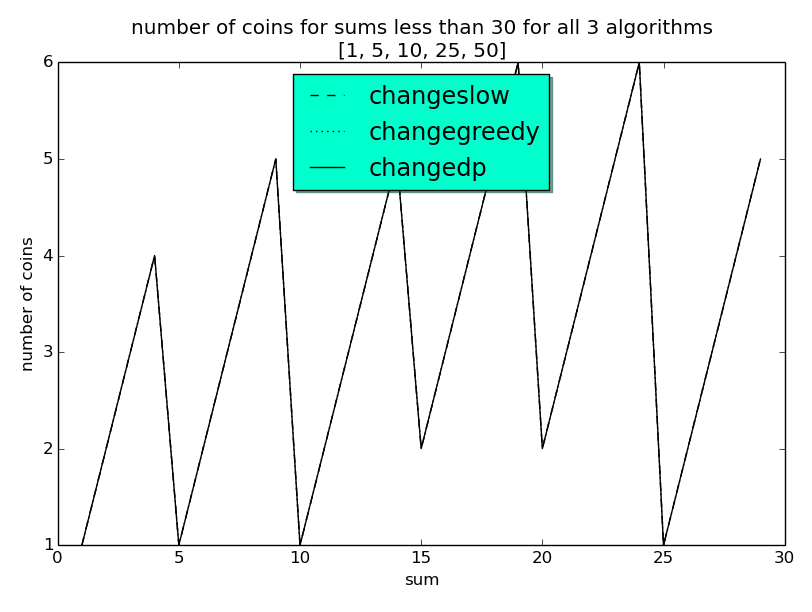
\includegraphics[width=\textwidth,height=\textheight,keepaspectratio]{q4_chart1.png}
\caption{Number of Coins, $Sum > 30$, V = 1,5,10,25,50}
\end{figure}

\autoref{q4_chart1b.png}
\begin{figure}[H!]
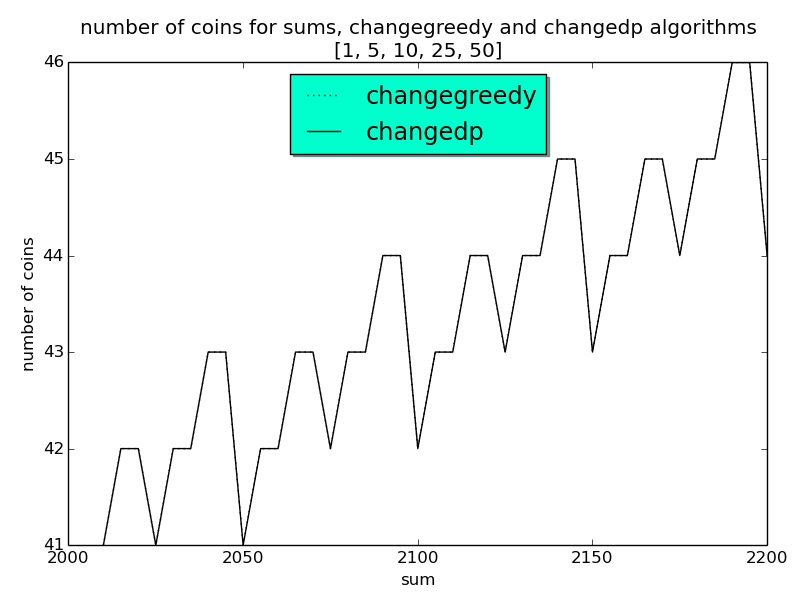
\includegraphics[width=\textwidth,height=\textheight,keepaspectratio]{q4_chart1b.png}
\caption{Number of Coins, $Sum > 2200$, V = 1,5,10,25,50}
\end{figure}

\autoref{q5_chart1.png}
\begin{figure}[H!]
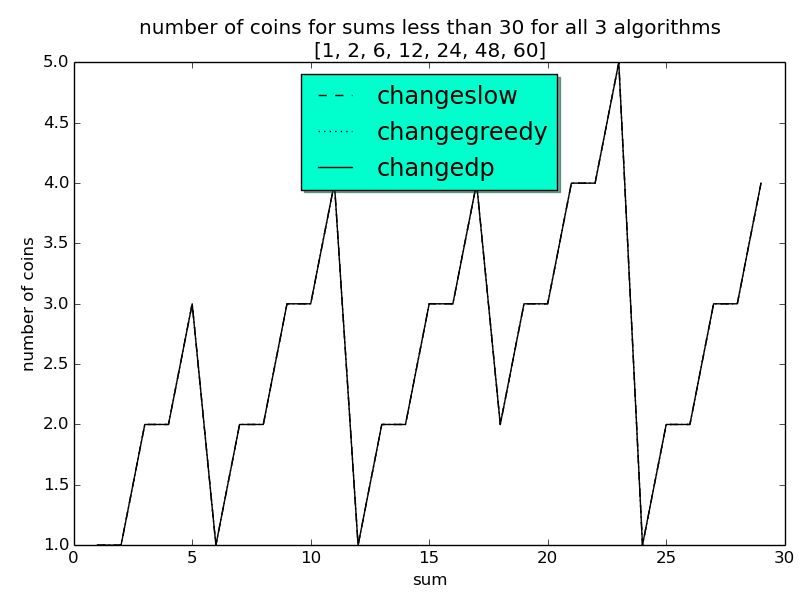
\includegraphics[width=\textwidth,height=\textheight,keepaspectratio]{q5_chart1.png}
\caption{Number of Coins, $Sum > 30$, V = 1,2,6,12,24,48,60}
\end{figure}

\autoref{q5_chart1b.png}
\begin{figure}[H!]
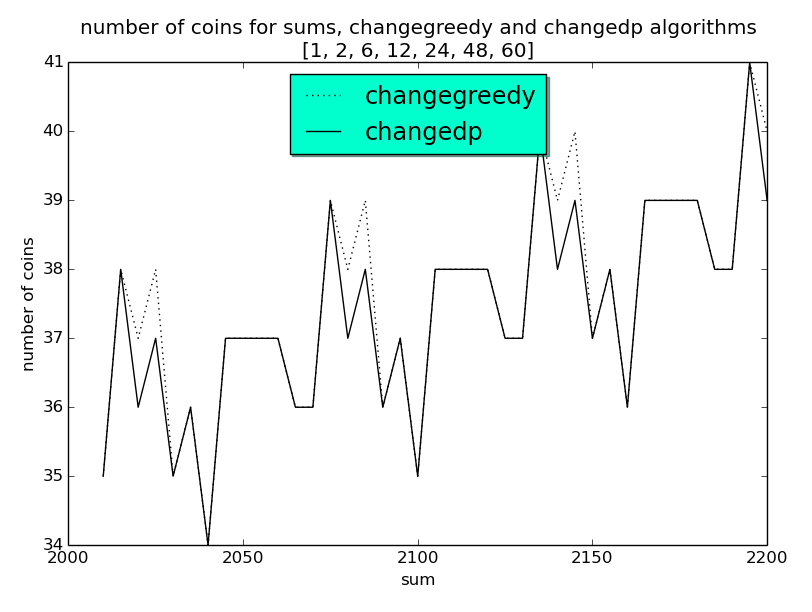
\includegraphics[width=\textwidth,height=\textheight,keepaspectratio]{q5_chart1b.png}
\caption{Number of Coins, $Sum > 2200$, V = 1,2,6,12,24,48,60}
\end{figure}

\autoref{q5_chart2.png}
\begin{figure}[H!]
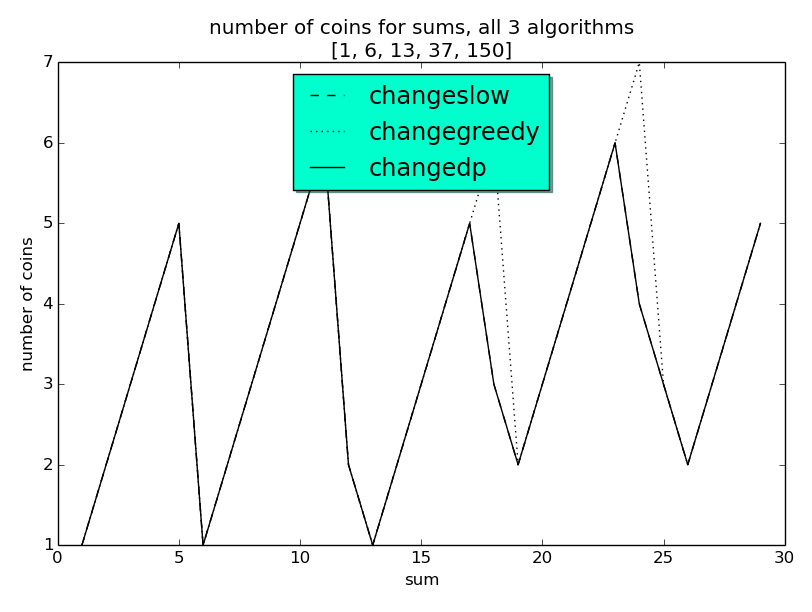
\includegraphics[width=\textwidth,height=\textheight,keepaspectratio]{q5_chart2.png}
\caption{Number of Coins, $Sum > 30$, V = 1,6,13,37,150}
\end{figure}

\autoref{q5_chart2b.png}
\begin{figure}[H!]
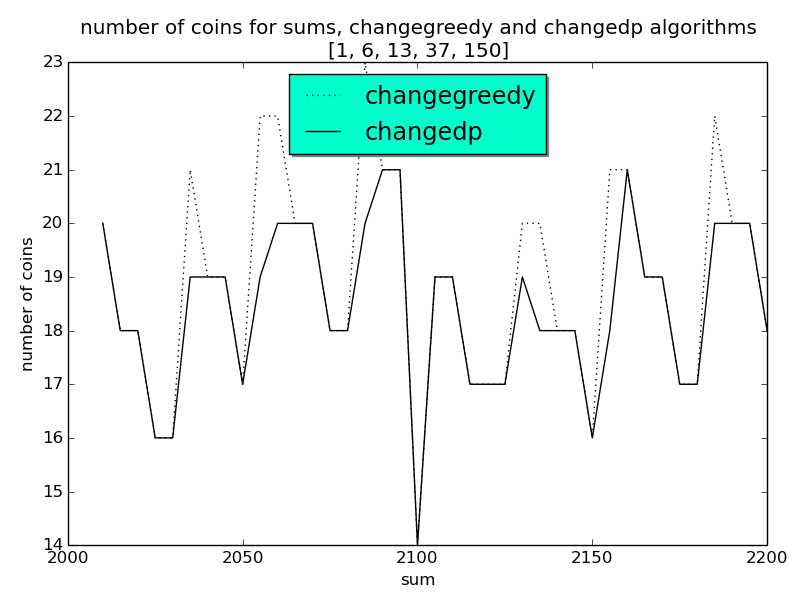
\includegraphics[width=\textwidth,height=\textheight,keepaspectratio]{q5_chart2b.png}
\caption{Number of Coins, $Sum > 2200$, V = 1,6,13,37,150}
\end{figure}

\autoref{q6_chart1.png}
\begin{figure}[H!]
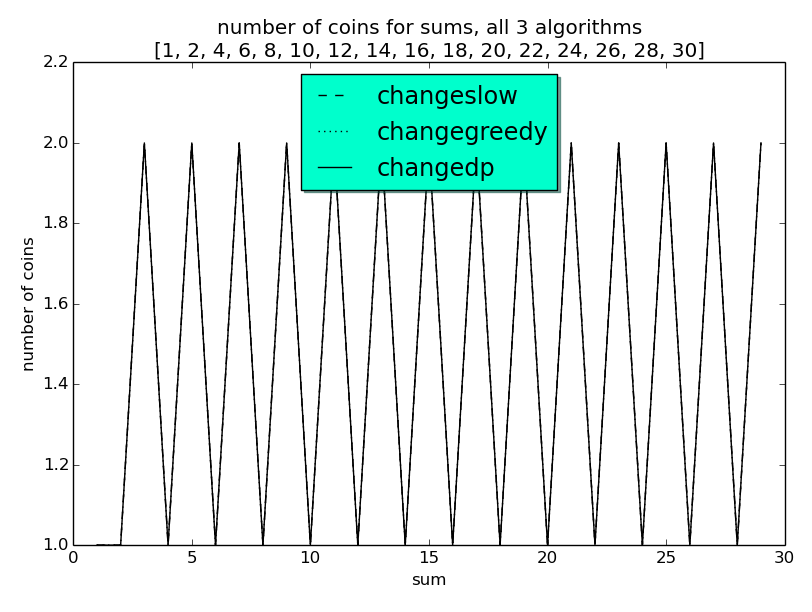
\includegraphics[width=\textwidth,height=\textheight,keepaspectratio]{q6_chart1.png}
\caption{Number of Coins, $Sum > 30$, V = 1,2,4,6,8,10,12,14,16,18,20,22,24,26,28,30}
\end{figure}

\autoref{q6_chart1b.png}
\begin{figure}[H!]
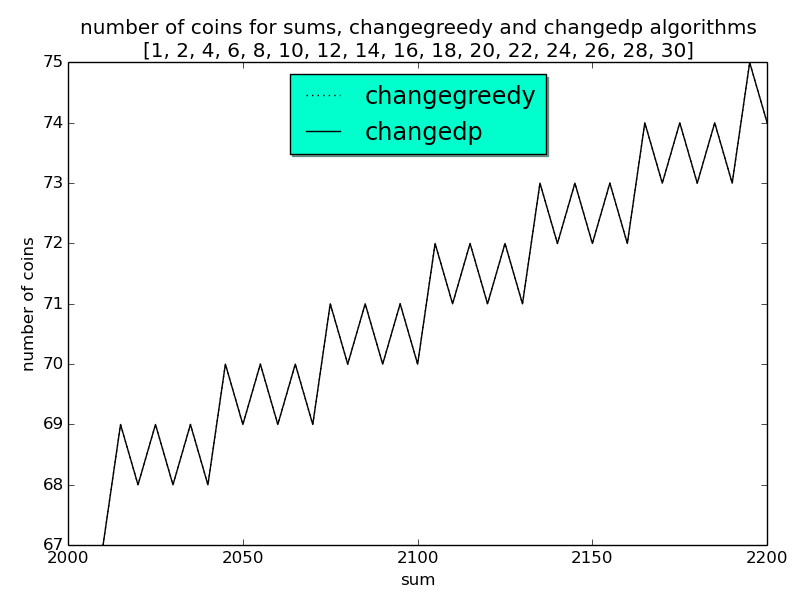
\includegraphics[width=\textwidth,height=\textheight,keepaspectratio]{q6_chart1b.png}
\caption{Number of Coins, $Sum > 2200$, V = 1,2,4,6,8,10,12,14,16,18,20,22,24,26,28,30}
\end{figure}

\autoref{q7c1.png}
\begin{figure}[H!]
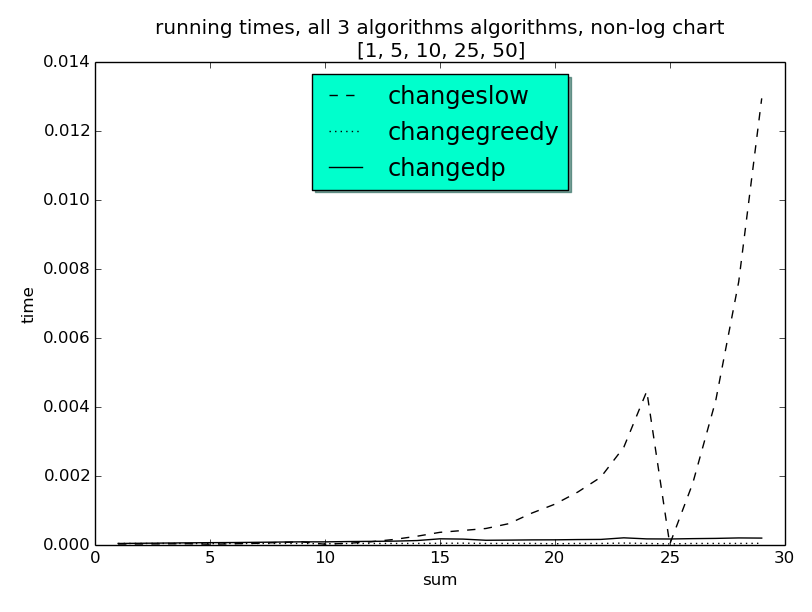
\includegraphics[width=\textwidth,height=\textheight,keepaspectratio]{q7c1.png}
\caption{Line of Best Fit, V = 1,5,10,25,50}
\end{figure}

\autoref{q7c1c.png}
\begin{figure}[H!]
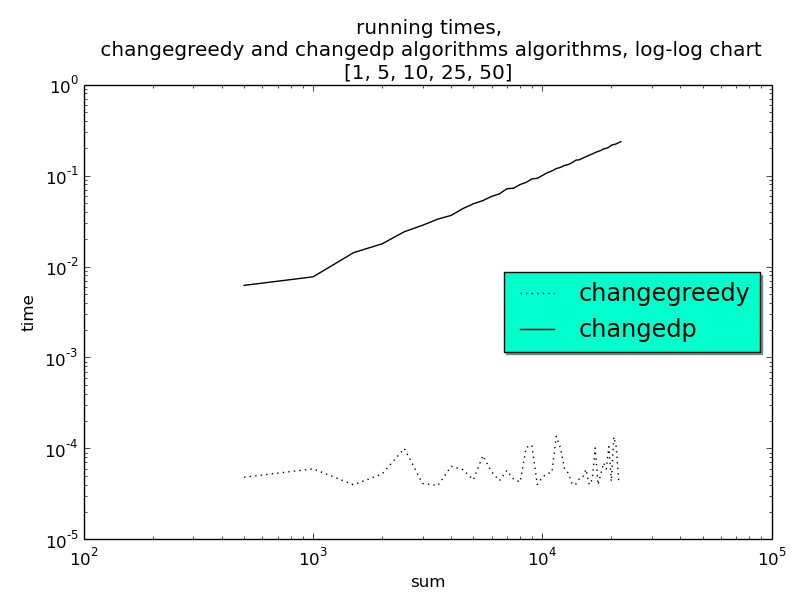
\includegraphics[width=\textwidth,height=\textheight,keepaspectratio]{q7c1c.png}
\caption{Log-Log, V = 1,5,10,25,50}
\end{figure}

\autoref{q7c2.png}
\begin{figure}[H!]
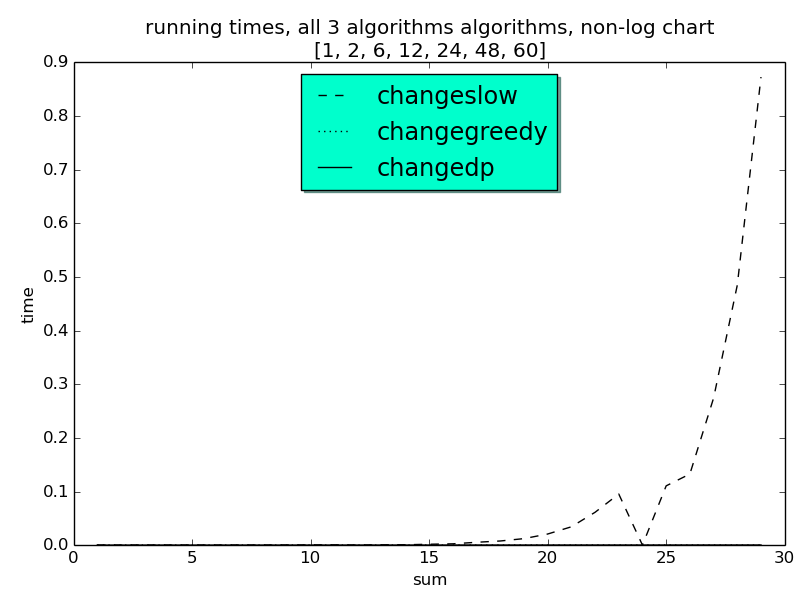
\includegraphics[width=\textwidth,height=\textheight,keepaspectratio]{q7c2.png}
\caption{Line of Best Fit, V = 1,2,6,12,24,48,60}
\end{figure}

\autoref{q7c2c.png}
\begin{figure}[H!]
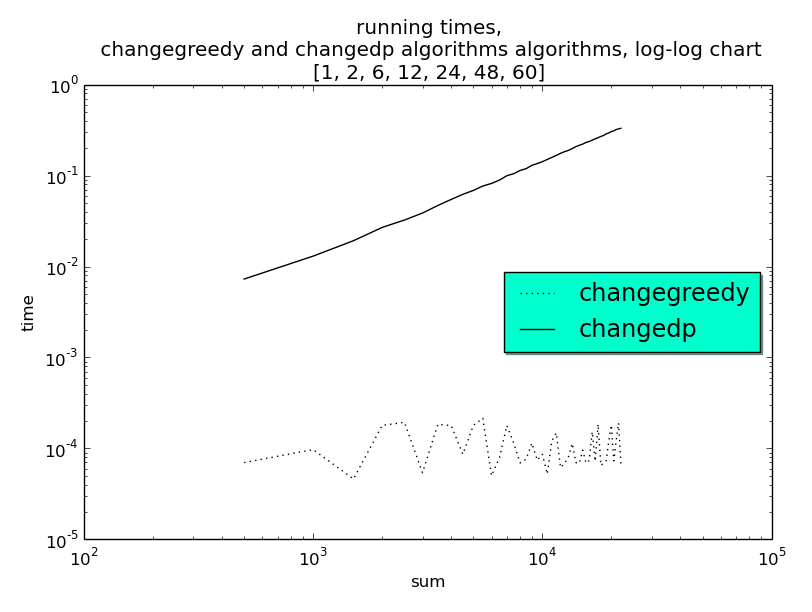
\includegraphics[width=\textwidth,height=\textheight,keepaspectratio]{q7c2c.png}
\caption{Log-Log, V = 1,2,6,12,24,48,60}
\end{figure}

\autoref{q7c3.png}
\begin{figure}[H!]
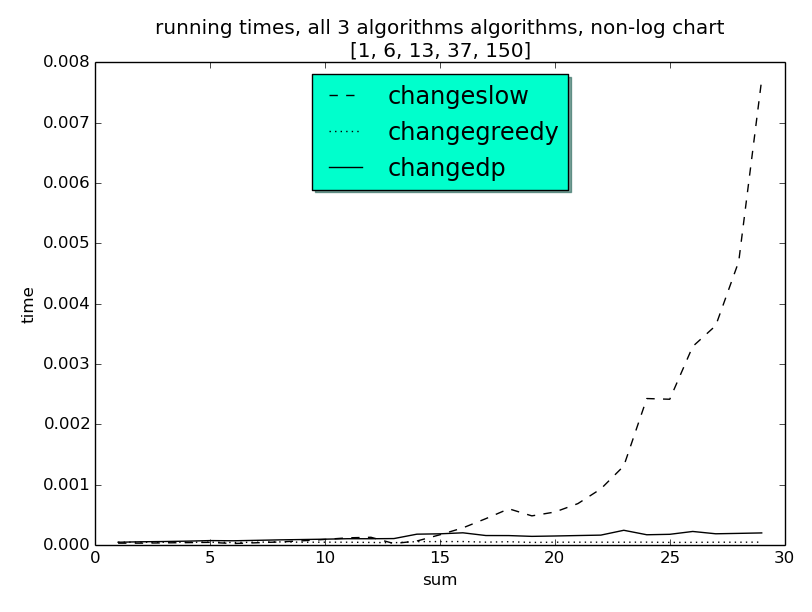
\includegraphics[width=\textwidth,height=\textheight,keepaspectratio]{q7c3.png}
\caption{Line of Best Fit, V = 1,6,13,37,150}
\end{figure}

\autoref{q7c3c.png}
\begin{figure}[H!]
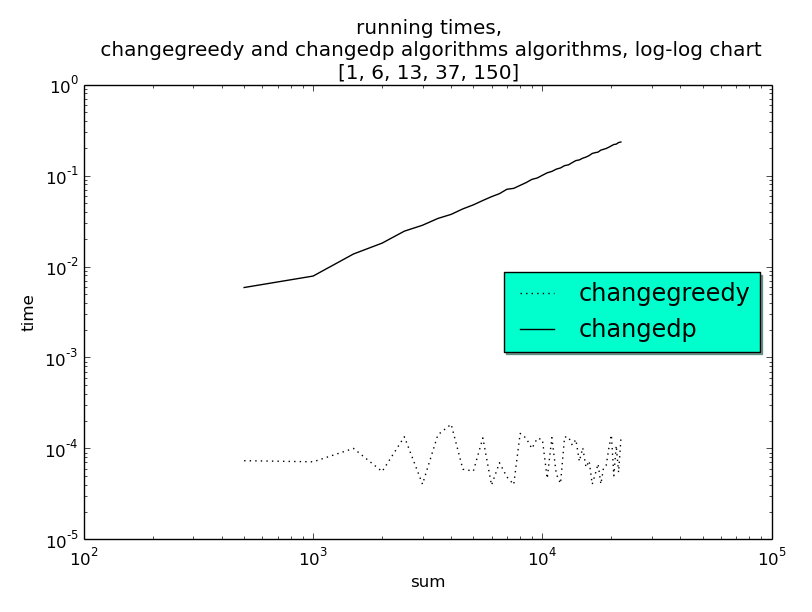
\includegraphics[width=\textwidth,height=\textheight,keepaspectratio]{q7c3c.png}
\caption{Log-Log, V = 1,6,13,37,150}
\end{figure}

\autoref{q7c4.png}
\begin{figure}[H!]
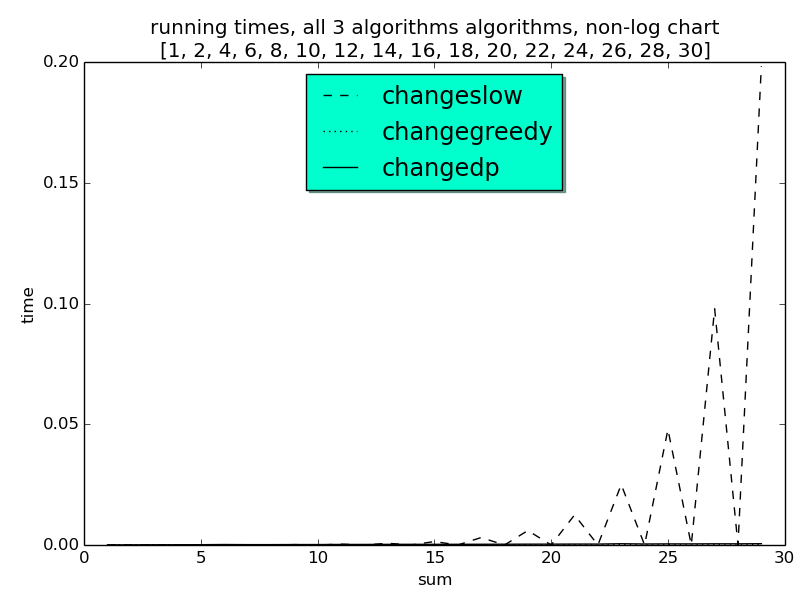
\includegraphics[width=\textwidth,height=\textheight,keepaspectratio]{q7c4.png}
\caption{Line of Best Fit, V = 1,2,4,6,8,10,12,14,16,18,20,22,24,26,28,30}
\end{figure}

\autoref{q7c4c.png}
\begin{figure}[H!]
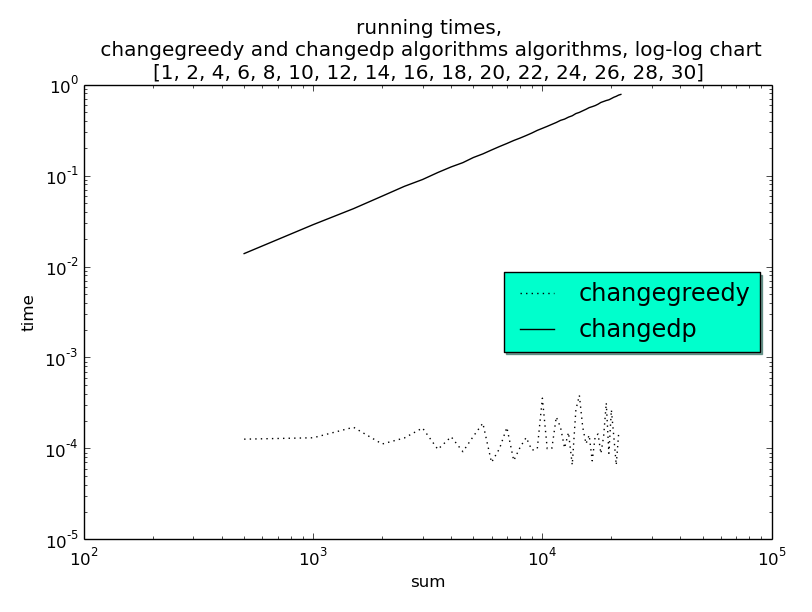
\includegraphics[width=\textwidth,height=\textheight,keepaspectratio]{q7c4c.png}
\caption{Log-Log, V = 1,2,4,6,8,10,12,14,16,18,20,22,24,26,28,30}
\end{figure}

\autoref{q8_chart1.png}
\begin{figure}[H!]
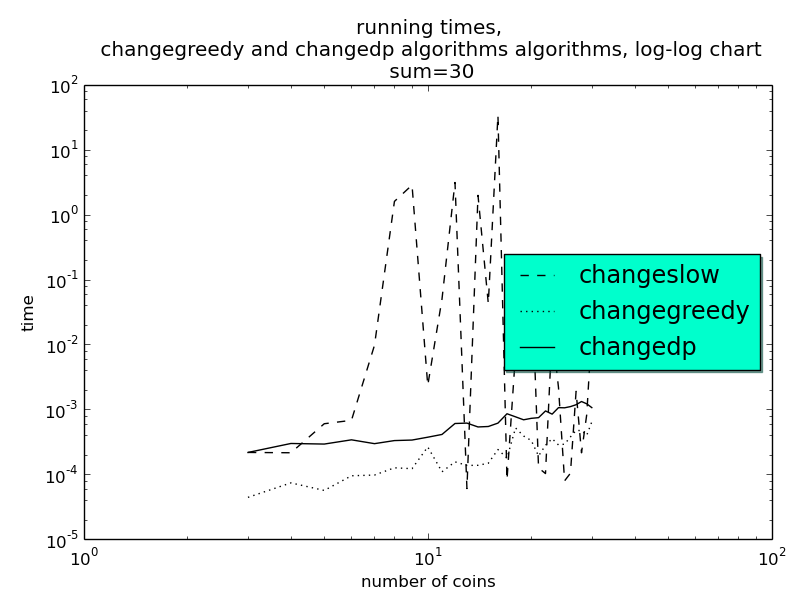
\includegraphics[width=\textwidth,height=\textheight,keepaspectratio]{q8_chart1.png}
\caption{Log-Log, Sum = 30}
\end{figure}

\autoref{q8_chart2.png}
\begin{figure}[H!]
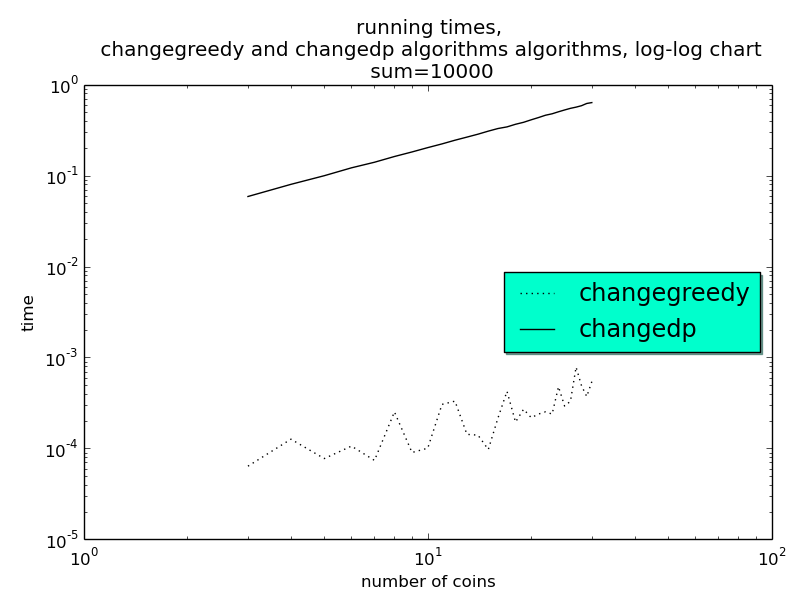
\includegraphics[width=\textwidth,height=\textheight,keepaspectratio]{q8_chart2.png}
\caption{Log-Log, Sum = 10,000}
\end{figure}

\autoref{q9chart1.png}
\begin{figure}[H!]
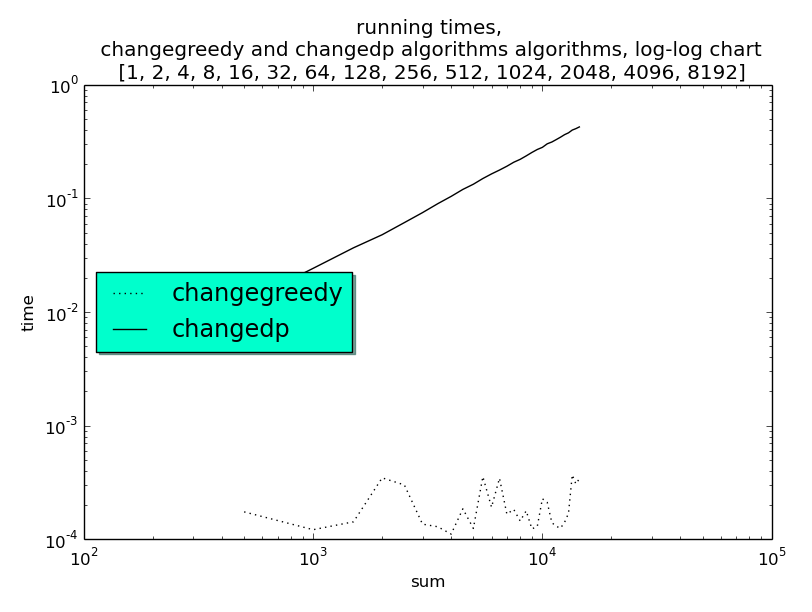
\includegraphics[width=\textwidth,height=\textheight,keepaspectratio]{q9chart1.png}
\caption{Long Term Comparison of Dynamic Programming and the Greedy Algorithm}
\end{figure}

\end{document}  